\documentclass[tikz, border=14pt]{standalone}
\usepackage{tikz}
\usepackage{amsmath}
\usepackage{amssymb}
\usetikzlibrary{positioning, fit, calc, shapes.geometric, arrows.meta, backgrounds}

%% ── Palette ─────────────────────────────────────────────────────────────────
\definecolor{nodeBlue}    {RGB}{219,234,254}   % concept node fill
\definecolor{nodeBlueBd}  {RGB}{ 37,099,235}   % concept node border
\definecolor{nodeGreen}   {RGB}{220,252,231}   % propagated node fill
\definecolor{nodeGreenBd} {RGB}{ 22,163, 74}   % propagated node border
\definecolor{cycleFill}   {RGB}{255,237,213}   % cycle edge warning fill
\definecolor{cycleBd}     {RGB}{234, 88, 12}   % cycle edge warning border
\definecolor{cycleText}   {RGB}{154, 52,  18}  % cycle text
\definecolor{cacheFill}   {RGB}{254,242,232}   % redis cache block fill
\definecolor{cacheBd}     {RGB}{217,119, 06}   % redis cache block border
\definecolor{visitFill}   {RGB}{254,226,226}   % visited-lock fill
\definecolor{visitBd}     {RGB}{220, 38, 38}   % visited-lock border
\definecolor{arrowGray}   {RGB}{100,116,139}   % standard arrows
\definecolor{propGreen}   {RGB}{ 22,163, 74}   % propagation arrow

%% ── Node styles ──────────────────────────────────────────────────────────────
\tikzset{
  concept/.style={
    circle, minimum size=2.6cm,
    align=center, font=\small\sffamily\bfseries,
    inner sep=4pt, draw, thick,
    fill=nodeBlue, draw=nodeBlueBd, text=nodeBlueBd
  },
  conceptG/.style={         % node that received propagation (green tint)
    concept,
    fill=nodeGreen, draw=nodeGreenBd, text=nodeGreenBd
  },
  %% small annotation box
  annot/.style={
    rectangle, rounded corners=4pt,
    align=center, font=\scriptsize\sffamily,
    inner sep=5pt, draw, thick
  },
  %% Redis cache side-block
  cache/.style={
    rectangle, rounded corners=6pt,
    align=left, font=\scriptsize\ttfamily,
    inner sep=8pt, draw, thick,
    fill=cacheFill, draw=cacheBd, text=black
  },
  %% Visited-lock label box
  visitlock/.style={
    rectangle, rounded corners=4pt,
    align=center, font=\scriptsize\sffamily\bfseries,
    inner sep=5pt, draw=visitBd, thick,
    fill=visitFill, text=visitBd
  },
  %% standard arrow
  arr/.style={
    -{Stealth[length=7pt,width=5pt]},
    thick, color=arrowGray
  },
  %% propagation arrow (green)
  arrP/.style={
    -{Stealth[length=7pt,width=5pt]},
    thick, color=propGreen
  },
  %% cycle / blocked arrow (dashed orange-red)
  arrC/.style={
    -{Stealth[length=7pt,width=5pt]},
    thick, color=cycleBd, dashed
  },
  lbl/.style={
    font=\scriptsize\sffamily, text=arrowGray,
    fill=white, inner sep=2pt, rounded corners=2pt
  },
  lblP/.style={         % propagation label (green)
    font=\scriptsize\sffamily, text=propGreen,
    fill=white, inner sep=2pt, rounded corners=2pt
  },
  lblC/.style={         % cycle label (red-orange)
    font=\scriptsize\sffamily, text=cycleBd,
    fill=white, inner sep=2pt, rounded corners=2pt
  }
}

\begin{document}
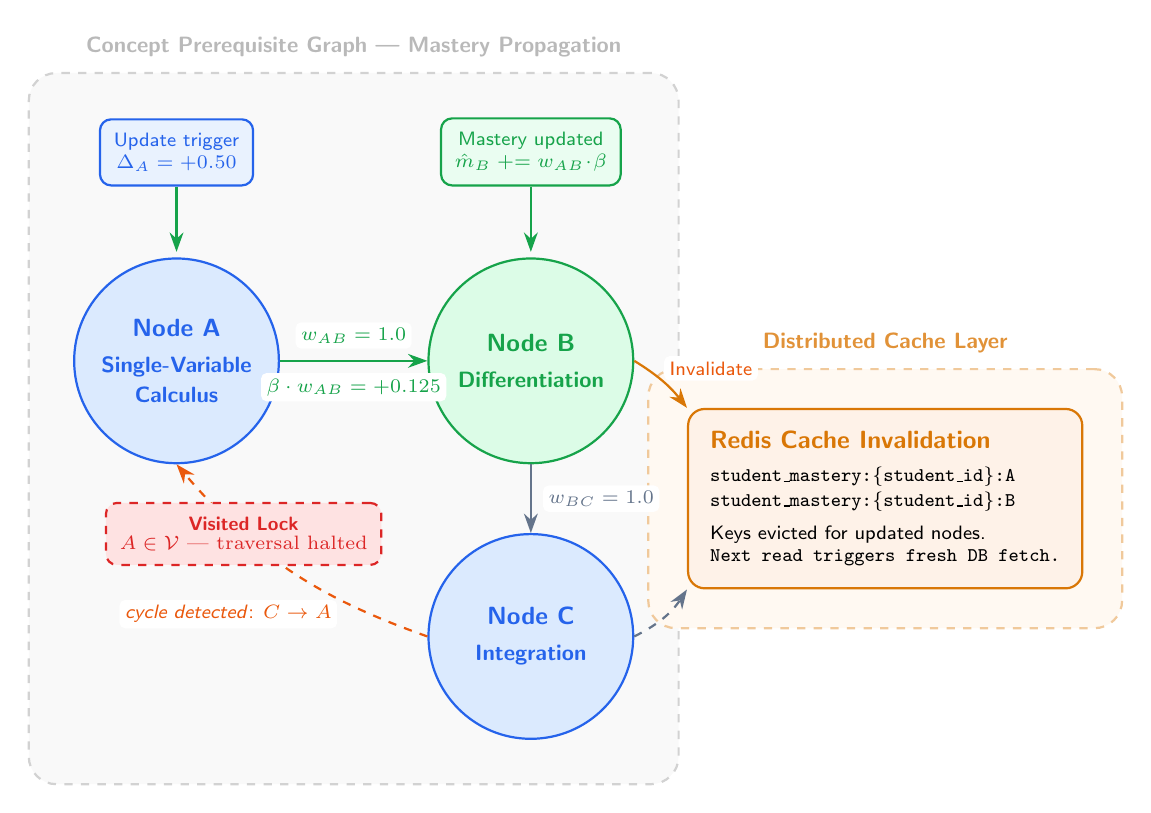
\begin{tikzpicture}

%% ═══════════════════════════════════════════════════════════
%%  CONCEPT NODES  (Triangle layout: A top-left, B top-right, C bottom-right)
%% ═══════════════════════════════════════════════════════════

\node[concept] (A) at (0, 3.5) {
  \textbf{Node A}\\[2pt]
  \footnotesize Single-Variable\\
  \footnotesize Calculus
};

\node[conceptG] (B) at (4.5, 3.5) {
  \textbf{Node B}\\[2pt]
  \footnotesize Differentiation
};

\node[concept] (C) at (4.5, 0) {
  \textbf{Node C}\\[2pt]
  \footnotesize Integration
};

%% ═══════════════════════════════════════════════════════════
%%  STEP 1 — Mastery update fires at A
%% ═══════════════════════════════════════════════════════════

\node[annot,
  fill=nodeBlue!60, draw=nodeBlueBd, text=nodeBlueBd,
  above=0.9cm of A
] (deltaA) {
  Update trigger\\
  $\Delta_A = +0.50$
};
\draw[arrP, shorten >=2pt] (deltaA.south) -- (A.north);

%% ═══════════════════════════════════════════════════════════
%%  EDGE  A -> B  (forward propagation)
%% ═══════════════════════════════════════════════════════════

\draw[arrP] (A.east) -- (B.west)
  node[lblP, midway, above=4pt]{$w_{AB} = 1.0$}
  node[lblP, midway, below=4pt]{$\beta \cdot w_{AB} = +0.125$};

%% ═══════════════════════════════════════════════════════════
%%  EDGE  B -> C  (standard vertical edge)
%% ═══════════════════════════════════════════════════════════

\draw[arr] (B.south) -- (C.north)
  node[lbl, midway, right=4pt]{$w_{BC} = 1.0$};

%% ═══════════════════════════════════════════════════════════
%%  CYCLE EDGE  C -> A  (back-edge, blocked by Visited Set)
%% ═══════════════════════════════════════════════════════════

%% Curved back-edge to avoid middle area
\draw[arrC] (C.west) to[bend left=15] 
  node[lblC, pos=0.3, below left] {\textit{cycle detected}: $C \to A$}
  node[visitlock, pos=0.7] (vlock) {
    Visited Lock\\[-1pt]
    \normalfont\scriptsize $A \in \mathcal{V}$ --- traversal halted
  }
  (A.south);

%% ═══════════════════════════════════════════════════════════
%%  PROPAGATION ANNOTATION on B
%% ═══════════════════════════════════════════════════════════

\node[annot,
  fill=nodeGreen!60, draw=nodeGreenBd, text=nodeGreenBd,
  above=0.9cm of B
] (propB) {
  Mastery updated\\
  $\hat{m}_B \mathrel{+}= w_{AB}\!\cdot\!\beta$
};
\draw[arrP, shorten >=2pt] (propB.south) -- (B.north);

%% ═══════════════════════════════════════════════════════════
%%  REDIS CACHE INVALIDATION BLOCK  (right side)
%% ═══════════════════════════════════════════════════════════

\node[cache] (redis) at (9.0, 1.75) {
  \normalfont\small\sffamily\bfseries\color{cacheBd}
  Redis Cache Invalidation\\[4pt]
  \texttt{student\_mastery:\{student\_id\}:A}\\[1pt]
  \texttt{student\_mastery:\{student\_id\}:B}\\[4pt]
  \normalfont\scriptsize\sffamily\color{black}
  Keys evicted for updated nodes.\\
  Next read triggers fresh DB fetch.
};

%% Arrow from B (updated node) to redis block
\draw[arr, color=cacheBd] (B.east) to[bend left=10] 
  node[lblC, midway, above right] {Invalidate} 
  (redis.north west);

%% Arrow from C to redis block (invalidation of downstream neighbor)
\draw[arr, color=arrowGray, dashed] (C.east) to[bend right=15] 
  (redis.south west);

%% ═══════════════════════════════════════════════════════════
%%  BACKGROUND CONTAINERS
%% ═══════════════════════════════════════════════════════════

\begin{scope}[on background layer]
  % Left container: Concept Graph
  \node[
    rectangle, rounded corners=10pt,
    fill=gray!5, draw=gray!35, dashed, thick,
    fit=(A)(B)(C)(deltaA)(propB)(vlock),
    inner sep=16pt
  ] (graphBox) {};
  
  % Right container: Distributed Cache Layer
  \node[
    rectangle, rounded corners=10pt,
    fill=orange!5, draw=cacheBd!40, dashed, thick,
    fit=(redis),
    inner sep=14pt
  ] (cacheBox) {};
\end{scope}

% Titles for containers
\node[
  font=\footnotesize\sffamily\bfseries, text=gray!55,
  above=2pt of graphBox.north, anchor=south
] {Concept Prerequisite Graph --- Mastery Propagation};

\node[
  font=\footnotesize\sffamily\bfseries, text=cacheBd!80,
  above=2pt of cacheBox.north, anchor=south
] {Distributed Cache Layer};

\end{tikzpicture}
\end{document}
